\documentclass{article}

\usepackage{fancyhdr} % Required for custom headers
\usepackage{lastpage} % Required to determine the last page for the footer
\usepackage{amsmath}
\usepackage{amsfonts}
\usepackage{dsfont}
\usepackage{graphicx}
\usepackage{subfigure}
\usepackage{listings}
\usepackage{booktabs}
\usepackage[hidelinks]{hyperref}
% \usepackage{epstopdf} uncomment this line if using MiKTeX

% Margins
\topmargin=-0.45in
\evensidemargin=0in
\oddsidemargin=0in
\textwidth=6.5in
\textheight=9.0in
\headsep=0.25in

\linespread{1.25} % Line spacing

% Set up the header and footer
\pagestyle{fancy}
\lhead{\authorName} % Top left header
\chead{\classID\ \hwTitle} % Top center header
\rhead{\studentID} % Top right header
\lfoot{} % Bottom left footer
\cfoot{} % Bottom center footer
\rfoot{Page\ \thepage\ of~\pageref{LastPage}} % Bottom right footer
\renewcommand{\headrulewidth}{0.4pt} % Size of the header rule
\renewcommand{\footrulewidth}{0.4pt} % Size of the footer rule

\setlength{\parindent}{0pt} % Removes all indentation from paragraphs

\setcounter{secnumdepth}{0} % Removes default section numbers
\newcounter{problemCounter} % Creates a counter to keep track of the number of problems

\newcommand{\problemName}{}
\newenvironment{problem}[1][Problem \arabic{problemCounter}]{
	\stepcounter{problemCounter} % Increase counter for number of problems
	\renewcommand{\problemName}{#1} % Assign \problemName the name of the problem
	\section{\problemName} % Make a section in the document with the custom problem count
}{}

\newcommand{\subproblemName}{}
	\newenvironment{subproblem}[1]{
	\renewcommand{\subproblemName}{#1} % Assign \subproblemName to the name of the section from the environment argument
	\subsection{\subproblemName} % Make a subsection with the custom name of the subsection
}{}

%----------------------------------------------------------------------------------------
%	MATH OPERATOR
%----------------------------------------------------------------------------------------

\DeclareMathOperator*{\argmin}{arg\,min}
\DeclareMathOperator*{\argmax}{arg\,max}

%----------------------------------------------------------------------------------------
%	NAME AND CLASS SECTION
%----------------------------------------------------------------------------------------

\newcommand{\hwTitle}{Assignment\ \#1} % Assignment title
\newcommand{\dueDate}{Thursday,\ February\ 21,\ 2017} % Due date
\newcommand{\classID}{ELEG\ 5491} % Course/Class
\newcommand{\authorName}{Kai Chen} % Your name
\newcommand{\studentID}{1155070509} % Your student ID

%----------------------------------------------------------------------------------------
%	TITLE PAGE
%----------------------------------------------------------------------------------------

\title{
	\vspace{2in}
	\textmd{\textbf{\classID:\ \hwTitle}}\\
	\normalsize\vspace{0.1in}\small{Due\ on\ \dueDate}
	\vspace{3in}
}

\author{\textbf{\authorName}}
\date{} % Insert date here if you want it to appear below your name

%----------------------------------------------------------------------------------------

\begin{document}
\maketitle
\setcounter{page}{0}
\thispagestyle{empty}
\newpage

%----------------------------------------------------------------------------------------
%	PROBLEM 1
%----------------------------------------------------------------------------------------

% To have just one problem per page, simply put a \clearpage after each problem

\begin{problem}

Cross entropy loss
\begin{align*}
\mathrm{CE} &= \frac{1}{N} \sum_{i=1}^{N} -\sum_{k=1}^{c} \mathds{1}(y_i^{(train)}=k)) \log(z_{i,k}) \\
&= \frac{1}{N} \sum_{i=1}^{N} -\log(z_{i,y_i^{(train)}})
\end{align*}

Negative log-likelihood on the training set
\begin{align*}
\mathcal{L} &= -\log P(Y^{(train)}|X^{(train)}) \\
&= -\sum_{i=1}^{N}\log P(y_i^{(train)}|x_i^{(train)}) \\
&= \sum_{i=1}^{N} -\log(z_{i,y_i^{(train)}})
\end{align*}

\end{problem}

%----------------------------------------------------------------------------------------
%	PROBLEM 2
%----------------------------------------------------------------------------------------

\begin{problem}

\begin{subproblem}{2.1}
	
\begin{align*}
f_{11}(x_1) &= x_1 - 0.5 \\
f_{12}(x_1) &= x_2 - 0.5 \\
g(h_{11}, h_{12}) &= h_{11} * h_{12}
\end{align*}

\end{subproblem}

\begin{subproblem}{2.2}
	
The network structure is shown in Figure~\ref{fig:2-2}, and the functions are
\begin{align*}
h_{11} &= \mathrm{abs}(x_1 - 1) \\
h_{12} &= \mathrm{abs}(x_2 - 1) \\
h_{21} &= h_{11} - 0.5 \\
h_{22} &= h_{12} - 0.5 \\
y &= h_{21} * h_{22}
\end{align*}
\begin{figure}[htbp]
	\centering
	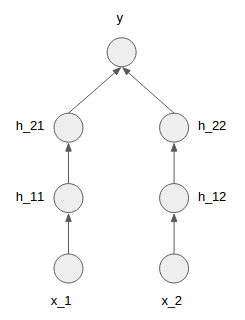
\includegraphics[width=2in]{image/2-2.png}
	\caption{Network structure}\label{fig:2-2}
\end{figure}

\end{subproblem}

\begin{subproblem}{2.3}

The decision boundary is shown in Figure~\ref{fig:2-3}.
\begin{figure}[htbp]
	\centering
	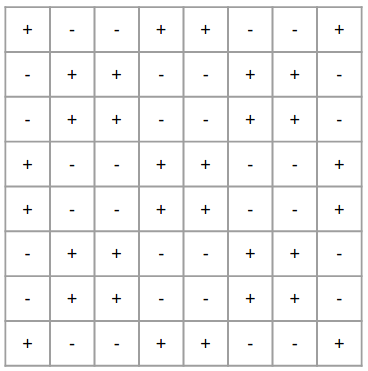
\includegraphics[width=2in]{image/2-3.png}
	\caption{Decision boundary}\label{fig:2-3}
\end{figure}

\end{subproblem}

\begin{subproblem}{2.4}

The network structure is shown in Figure~\ref{fig:2-4}.

\begin{figure}[htbp]
	\centering
	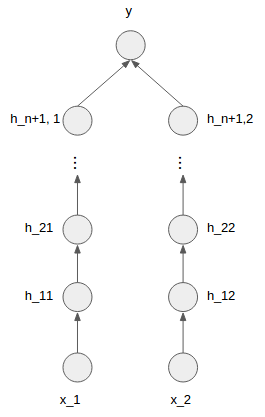
\includegraphics[width=2in]{image/2-4.png}
	\caption{Network structure}\label{fig:2-4}
\end{figure}

\begin{align*}
h_{11} &= \mathrm{abs}(x_1 - 2^{n-1}) \\
h_{12} &= \mathrm{abs}(x_2 - 2^{n-1}) \\
h_{k+1,1} &= \mathrm{abs}(h_{k,1} - 2^{n-k-1}) \text{ for } k \text{ in } 1,2,\dots,n-1 \\
h_{k+1,2} &= \mathrm{abs}(h_{k,2} - 2^{n-k-1}) \text{ for } k \text{ in } 1,2,\dots,n-1 \\
h_{n+1,1} &= h_{n,1} - 0.5 \\
h_{n+1,2} &= h_{n,2} - 0.5 \\
y &= h_{n+1,1}h_{n+1,2}
\end{align*}

\end{subproblem}

\begin{subproblem}{2.5}
	
The network structure is shown in Figure~\ref{fig:2-5}. The fianl transform function is
\[
y = \prod_{k=1}^{2^{n+1}-1}(x_1-\frac{k}{2})(x_2-\frac{k}{2})
\]

\begin{figure}[htbp]
	\centering
	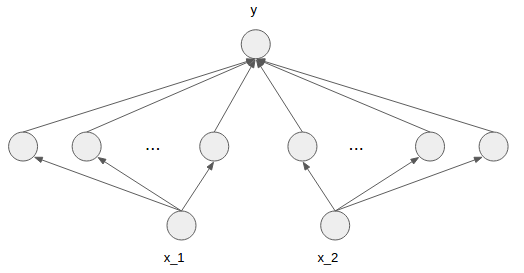
\includegraphics[width=3in]{image/2-5.png}
	\caption{1-hidden-layer structure}\label{fig:2-5}
\end{figure}


\end{subproblem}


\end{problem}

%----------------------------------------------------------------------------------------
%	PROBLEM 3
%----------------------------------------------------------------------------------------

\begin{problem}

The receptive field of a neuron as the output of the pooling layer in (a) is $8\times8$, in (b) is $13\times13$.

\end{problem}

%----------------------------------------------------------------------------------------
%	PROBLEM 4
%----------------------------------------------------------------------------------------

\begin{problem}

\begin{subproblem}{4.1}

\begin{align*}
[[L_tf]*w](x) &= \sum_{y\in\mathbb{Z}^2}\sum_{k=1}^{K}[L_tf]_k(y)w_k(y-x) \\
&= \sum_{y\in\mathbb{Z}^2}\sum_{k=1}^{K}f_k(y-t)w_k(y-x) \\
&= \sum_{y+t\in\mathbb{Z}^2}\sum_{k=1}^{K}f_k(y)w_k(y-(x-t)) \\
&= \sum_{y\in\mathbb{Z}^2}\sum_{k=1}^{K}f_k(y)w_k(y-(x-t)) \\
&= [L_t[f*w]](x)
\end{align*}

\end{subproblem}

\begin{subproblem}{4.2}

\begin{align*}
[[L_\mathbf{R}f]*w](x) &= \sum_{y\in\mathbb{Z}^2}\sum_{k=1}^{K}[L_\mathbf{R}f]_k(y)w_k(y-x) \\
&= \sum_{y\in\mathbb{Z}^2}\sum_{k=1}^{K}f_k(\mathbf{R}^{-1}y)w_k(y-x) \\
&= \sum_{\mathbf{R}y\in\mathbb{Z}^2}\sum_{k=1}^{K}f_k(y)w_k(\mathbf{R}y-x) \\
&= \sum_{y\in\mathbb{Z}^2}\sum_{k=1}^{K}f_k(y)w_k\mathbf{R}(y-\mathbf{R}^{-1}x) \\
&= L_\mathbf{R}\sum_{\mathbf{R}y\in\mathbb{Z}^2}\sum_{k=1}^{K}f_k(y)w_k\mathbf{R}(y-x) \\
&= L_\mathbf{R}[f*[L_{\mathbf{R}^{-1}}w]](x)
\end{align*}

\end{subproblem}

\begin{subproblem}{4.3}

\begin{align*}
[[L_\mathbf{u}f]*w](\mathbf{g}) &= \sum_{\mathbf{h}\in G}\sum_{k=1}^{K}[L_\mathbf{u}f]_k(\mathbf{h})w_k(\mathbf{g}^{-1}\mathbf{h}) \\
&= \sum_{\mathbf{h}\in G}\sum_{k=1}^{K}f_k(\mathbf{u}^{-1}\mathbf{h})w_k(\mathbf{g}^{-1}\mathbf{h}) \\
&= \sum_{\mathbf{u}\mathbf{h}\in G}\sum_{k=1}^{K}f_k(\mathbf{h})w_k(\mathbf{g}^{-1}\mathbf{u}\mathbf{h}) \\
&= \sum_{\mathbf{h}\in G}\sum_{k=1}^{K}f_k(\mathbf{h})w_k((\mathbf{u}^{-1}\mathbf{g})^{-1}\mathbf{h}) \\
&= [L_\mathbf{u}[f*w]](\mathbf{g})
\end{align*}

\end{subproblem}

\end{problem}

\end{document}
